\chapter{Query templates}\label{chapter:templates}



The translation is based on the idea of creating queries that reproduce callstack-growth and evaluation. The form of these queries is always identical -- only the expressions that are evaluated at distinct points are dependant on the input UDF. In this chapter I present the templates that are used to create and evaluate the callgraph.

The templates are given in a macro-style where the required data is given as arguments. Filling out the templates involves neither analyzing nor data extraction. All required information, predicates, scenarios etc. is present in an intermediate representation of the UDF (\autoref{intermed:fib_output}). The generation of the intermediate representation will be explained in \autoref{chapter:analysis}.

\begin{figure}[h!]
    \centering\small
    
    \begin{align*}
\Big(&\big\{&\big\langle~&\text{pred}:     &\mintinline{postgresql}{SELECT ($1 = 0)}                  &\\
    &      &    ,~      &\text{query}:    &\mintinline{postgresql}{SELECT 0}                          & \big\rangle \big\}\\
, ~ &\big\{&\big\langle~&\text{pred}:     &\mintinline{postgresql}{SELECT (NOT $1 = 0) AND ($1 = 1)}&\\
    &      &    ,~      &\text{query}:    &\mintinline{postgresql}{SELECT 1 + fib(0)}&    \\
    &      &    ,~      &\text{callsites}:&\langle \text{id}: 1,~\text{args}: (\mintinline{postgresql}{SELECT 0})\big\rangle & \big\rangle\\
    &      &\big\langle~&\text{pred}:     &\mintinline{postgresql}{SELECT (NOT $1 = 0) AND (NOT $1 = 1)}&\\
    &      &    ,~      &\text{query}:    &\mintinline{postgresql}{SELECT fib($1 - 1) + fib($1 - 2)}&\\
    &      &    ,~      &\text{callsites}:&\langle \text{id}: 2,~\text{args}: (\mintinline{postgresql}{SELECT $1 - 1})\rangle &,\\
    &      &            &                 &\langle \text{id}: 3,~\text{args}: (\mintinline{postgresql}{SELECT $1 - 2})\rangle & \big\rangle\big\} \Big)
    \end{align*}
    \caption{Intermediate representation of \texttt{fib(int)} used as data source for the templates. Not shown but also required are the name of the UDF and its argument- and return-types.}
    \label{intermed:fib_output}
\end{figure}



% Two phases: Callgraph growth and callstack evaluation
There are two main phases -- callgraph creation and callgraph evaluation -- which are implemented as two CTEs, \texttt{callgraph} and \texttt{evaluation}. The final query selects the desired final output from the evaluation-CTE. \autoref{fig:standard_template_structure} illustrates the very high level idea of the standard translation template.

\begin{figure}[h!]
    \centering
    \begin{cminted}{postgresql}
CREATE FUNCTION fn(INT) RETURNS INT AS $$
  WITH RECURSIVE
    callstack(in_1, callsite_id, out_1) AS (
      <collect initial callsites>
        UNION
      <collect subsequent callsites>
    ),
    evaluation(in_1, result) AS (
      <evaluate basecases>
        UNION ALL
      <evaluate recursive scenarios>
    )
  SELECT e.result FROM evaluation e WHERE (e.in_1) = ($1)
$$ LANGUAGE SQL;
\end{cminted}
    \caption{High-level structure of the standard query template (simplified).}
    \label{fig:standard_template_structure}
\end{figure}

% Special care needs to be taken to behave not only in terms of result values, but also in terms of termination.
Special care needs to be taken to behave like the original function in terms of termination. Call-loops in the original function lead to an infinite growing callstack, causing nontermination. By using memoization in the translation, this does not happen in our template, consequently we have to manually detect and initiate nontermination.

In this chapter I provide a number of "template-macros" with respect to the running example of the unary function \texttt{fib}. Actually, each macro would need to generalize over the number of arguments, but this would clutter difficult spots with excessive notation. Instead, I state here once the required steps to generalize the macros for unary to n-ary functions.

To generalize the macros to more arguments the following things need to be done:
\begin{itemize}
    \item Instead of a single column \texttt{in\_1} or \texttt{out\_1}, we need further columns \texttt{in\_2, ..., in\_n} and \texttt{out\_2, ..., out\_n}.
    \item Whenever we match tables by their arguments, eg. \texttt{(c.in\_1) = (e.out\_1)} this needs to be altered analogous: \texttt{(c.in\_1, c.in\_2, ..., c.in\_n) = (e.out\_1, e.out\_2, ..., out\_n)}.
    \item The same applies whenever replacing an UDF argument \texttt{\$1} in \texttt{q} by \texttt{x1}: \texttt{q[x1/\$1]} needs to become \texttt{q[x1/\$1, x2/\$1, ..., xn/\$n]}.
\end{itemize}

For full examples with more than one argument see the appendix \autoref{???}. 

\section{Callgraph discovery}

Starting with the original arguments of the UDF-invocation, the current evaluation scenario is detected and the contained callsites are discovered. The arguments passed to the newly discovered callsites are evaluated independently and used to recursively collect subsequent calls.

\begin{figure}[h!]\small
    \begin{minipage}[b]{.5\linewidth}
    \centering
    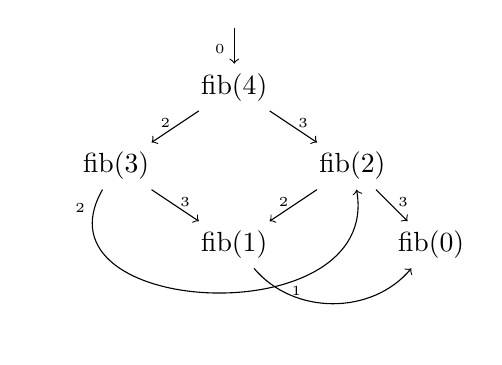
\begin{tikzpicture}
% nodes
\node (f4)     at (2.5, 2) {fib(4)};
    \node (f3) at (1, 1) {fib(3)};
        \node (f1) at (2.5, 0) {fib(1)};
    \node (f2) at (4, 1) {fib(2)};
        \node (f0) at (5, 0) {fib(0)};
% arrows
\draw[<-] (f4) -- node[pos=0.4, left, label distance=5mm]{\tiny{0}} +(0, 0.75);

\draw[->] (f4) -- node[pos=0.4, left, label distance=5mm]{\tiny{2}} (f3);
\draw[->] (f4) -- node[pos=0.4, right, label distance=5mm]{\tiny{3}} (f2);

    \draw[->, bend right=100, out=240, looseness=1.5] (f3) to node[pos=0.05, left, label distance=5mm]{\tiny{2}} (f2);
    \draw[->] (f3) -- node[pos=0.4, right, label distance=5mm]{\tiny{3}} (f1);
    \draw[->] (f2) -- node[pos=0.4, left, label distance=5mm]{\tiny{2}} (f1);
        \draw[->, bend right=50] (f1) to node[pos=0.2, right, label distance=5mm]{\tiny{1}} (f0);
    \draw[->] (f2) -- node[pos=0.4, right, label distance=5mm]{\tiny{3}} (f0);
\end{tikzpicture}
    \subcaption{Callgraph during execution}\label{fig:fib_callstack_graph}
    \end{minipage}%
    \begin{minipage}[b]{.5\linewidth}
    \centering
    
    \begin{tabular}{@{}|c|c|c|@{}}
  \tabname{2}{\strut\texttt{\,callgraph\,}} \\
  \colhd{in\_1} & \colhd{callsite\_id} & \colhd{out\_in} \\
        \texttt{NULL} & \texttt{0} & \texttt{4}\\
        \hline
        \texttt{4} & \texttt{2} & \texttt{3}\\
        \texttt{4} & \texttt{3} & \texttt{2}\\
        \hline
        \texttt{3} & \texttt{2} & \texttt{2}\\
        \texttt{3} & \texttt{3} & \texttt{1}\\
        \texttt{2} & \texttt{2} & \texttt{1}\\
        \texttt{2} & \texttt{3} & \texttt{0}\\
        \hline
        \texttt{1} & \texttt{1} & \texttt{0}\\
        \hline
\end{tabular}
    \subcaption{Tabular representation of the callstack}\label{fig:fib_callstack_table}
    \end{minipage}
    \caption{Callgraph of \texttt{fib(4)} (a) and its tabular representation as generated by the \texttt{callstack}-CTE (b). Each edge represents a callsite.}\label{fig:fib_callstack}
\end{figure}

The callgraph-CTE creates a direct encoding of the actual callstack-tree but collapses identical nodes into one, resulting in a Directed Acyclic Graph (DAG) if the recursion contains no loops (\autoref{fig:fib_callstack}). Each row depicts an edge between two nodes including the label. Nodes of the callgraph correspond to recursive calls, identified by their arguments, one column per argument. Moreover, the arguments of the caller and callee and the id of the callsite are noted. Callsite ids are used to associate callsites to scenarios.

%\subsection{Collecting callsite arguments}

The callgraph is created by an self-referential CTE. The base query and the self-referential query of the CTE are nearly identical. Each callsite has an own query returning a single row (input arguments, callsite id, callsite arguments) if the predicate of its scenario is fulfilled. The template is given in \autoref{marco:collect_call_maybe}.
The predicate acts as guard to add purely callsites of the current evaluation scenario. Only if the predicate is fulfilled, any row is returned. For example, the query that returned the third row in \autoref{fig:fib_callstack_table} is generated by \mintinline{postgresql}{<collect_call_maybe(d.out_1, p2, <callsite id: 3, arg_1: (SELECT $1 - 2)>)>}.

\begin{figure}[h!]\centering
    \begin{minted}{postgresql}
    <collect_call_maybe(in_arg_1, predicate, callsite)>
        := SELECT
             in_arg_1                    AS in_1, 
             callsite.id                 AS callsite_id,
             callsite.arg_1[in_arg_1/$1] AS out_1
           FROM predicate AS p(is_true)
           WHERE p.is_true
    \end{minted}
  \caption{Pseudocode to generate a single call to the callgraph-table. $q[y/x]$ denots the operation of replacing $y$ for $x$ in $q$. For \texttt{in\_arg\_1} it is used in the beginning \texttt{\$1} and later references to preceding arguments from the table.}
  \label{marco:collect_call_maybe}
\end{figure}

The macro from \autoref{marco:collect_call_maybe} creates only a query returning one or none rows. To collect \textit{all} callsites the query needs to test all callsites of all scenarios (\autoref{macro:collect_calls}). As all callsites within a scenario depend on the same predicate the scenario-predicate can be pulled up into a CTE to avoid multiple evaluations.

\begin{figure}[h!]\centering\small
    \begin{minted}{postgresql}
    <collect_calls(in_arg_1, scenarios)> :=
        WITH p1 AS (scenarios[1].predicate)[in_arg_1/$1],
             p2 AS (scenarios[2].predicate)[in_arg_1/$1]
             
        -- Scenario 1
        (   -- Callsite 1
            <collect_call_maybe(in_arg_1, p1, scenarios[1].callsites[1])>   )
        
        UNION
        
        -- Scenario 2
        (   -- Callsite 2
            <collect_call_maybe(in_arg_1, p2, scenarios[2].callsites[1])>
          UNION
            -- Callsite 3
            <collect_call_maybe(in_arg_1, p2, scenarios[2].callsites[2])>   )
\end{minted}
  \caption{All callsites of all scenarios needs to be tested to cover the entire UDF.}
  \label{macro:collect_calls}
\end{figure}

With the query generated by \texttt{<collect\_calls(\$1, scenarios)>} all callsites of the initial UDF invocation are obtained. Subsequent levels of the callgraph can be collected recursively by using the \texttt{out\_1}-column from the previous iteration instead of \texttt{\$1}. For each callsite from the previous iteration the according evaluation scenario needs to be detected to collect new callsites. This for-each behaviour is implemented by \texttt{LATERAL} in the template for \texttt{callgraph} (\autoref{macro:callgraph}).

\begin{figure}[h!]\centering
\begin{cminted}{postgresql}
<callgraph(rec_scenarios)> :=
  (
    (SELECT NULL, 0, $1) -- add original call
      UNION ALL
    <collect_calls($1, rec_scenarios)> 

  ) UNION (
    SELECT
      new_calls.*
    FROM
      callgraph AS c, LATERAL (
        <collect_calls(c.out_1, rec_scenarios)>
      ) AS new_calls
  )
\end{cminted}
  \caption{Macro to generate the \texttt{callgraph}-CTE.}
  \label{macro:callgraph}
\end{figure}


\iffalse
\begin{figure}[h!]
    \centering
    \bgroup
\def\arraystretch{1.5}
\begin{tabular}{|c|}\hline
%\footnotesize\mintinline{postgresql}{in_args := $1 / SELECT c.call_args FROM callstack c}\\
\begin{tabular}{|l|}\hline
    \footnotesize{Scenario 1}\\
    \begin{tabular}{|l|}\hline
        \footnotesize{Callsite 1}\\
        \footnotesize\mintinline{postgresql}{SELECT in_args, callsite.id, callsite.args AS call_args}\\[-5pt]
        \footnotesize\mintinline{postgresql}{  FROM scenario.pred p WHERE p.v}\\
    \hline \end{tabular}\\
    \mintinline{postgresql}{UNION}\\
    \begin{tabular}{|l|}\hline
        \footnotesize{Callsite 2}\\
        \footnotesize\mintinline{postgresql}{SELECT in_args, callsite.id, callsite.args AS call_args}\\[-5pt]
        \footnotesize\mintinline{postgresql}{  FROM scenario.pred p WHERE p.v}\\
    \hline \end{tabular}\\[2mm]
\hline \end{tabular}\\
    \mintinline{postgresql}{UNION}\\
\begin{tabular}{|l|}\hline
    \footnotesize{Scenario 2}\\
    \begin{tabular}{|l|}\hline
        \footnotesize{Callsite 3}\\
        \footnotesize\mintinline{postgresql}{SELECT in_args, callsite.id, callsite.args AS call_args}\\[-5pt]
        \footnotesize\mintinline{postgresql}{  FROM scenario.pred p WHERE p.v}\\
    \hline \end{tabular}\\[2mm]
\hline \end{tabular}
\\[6mm]
\hline
\end{tabular}
\egroup
    \caption{Structure of the callstack CTE. In the beginning, the original parameters \$1 are used. The recursive step iterates over all newly discovered calls.}
    \label{discovery_strucutre}
\end{figure}
\fi

For a examples of complete \texttt{callgraph}-CTEs, see \autoref{appendix:translations} in the appendix.

Callgraph growth ends as soon as no recursive scenario is applicable for any newly discovered callsites, ie. all callsites lead to basecases. In this case the new iteration contains no rows causing \texttt{WITH RECURSIVE} to stop.

\section{Callgraph evaluation}
% Evaluation starts bottom up at the leaves of the callstack
Evaluation starts bottom up from the leafs of the callgraph. Scenarios are evaluated by replacing their original arguments with references to the arguments from the callgraph (\autoref{macro:single_basecase}). Scenarios may depend on other scenarios that need to be evaluated first. If all dependencies of a scenario are evaluated, the scenario can be evaluated itself. Nonrecursive scenarios have no dependencies and can therefore be evaluated straight ahead. From those results of the basecases the evaluation continues. Eventually, the desired result can be selected.

\begin{figure}[h!]\small
    \begin{minipage}[b]{.45\linewidth}\small
    \centering
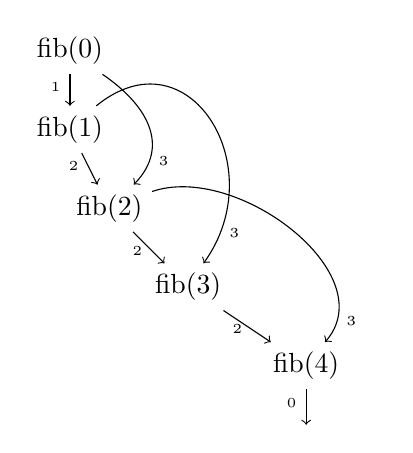
\begin{tikzpicture}
% nodes
\node (n4) at (2.5, -2) {fib(4)};
\node (n3) at (1, -1) {fib(3)};
\node (n2) at (0, 0) {fib(2)};
\node (n1) at (-0.5, 1) {fib(1)};
\node (n0) at (-0.5, 2) {fib(0)};
% arrows
\draw[->] (n0)     to node[pos=0.4,left] {\tiny{1}} (n1);
\draw[->, bend left=40, looseness=1.2, in=120] (n0)     to node[pos=0.8,right] {\tiny{3}} (n2);
\draw[->] (n1)     to node[pos=0.4,left] {\tiny{2}} (n2);
\draw[->, bend left=70, looseness=1.6, out=95] (n1)     to node[pos=0.9,right] {\tiny{3}} (n3);
\draw[->] (n2)     to node[pos=0.6,left] {\tiny{2}} (n3);
\draw[->, bend left=60, looseness=1, in=90] (n2)     to node[pos=0.9,right] {\tiny{3}} (n4);
\draw[->] (n3)     to node[pos=0.6,left] {\tiny{2}} (n4);
\draw[->] (n4)     to node[pos=0.4,left] {\tiny{0}} +(0, -0.75);
\end{tikzpicture}
    \subcaption{}\label{}
    \end{minipage}%
    \hfill
    \begin{minipage}[b]{.45\linewidth}\small
    \centering
    \begin{tabular}{@{}|c|c|@{}}
  \tabname{2}{\strut\texttt{\,evaluation\,}} \\
  \colhd{in\_1} & \colhd{result} \\
  \texttt{0} & \texttt{0} \\\hline
  \texttt{1} & \texttt{1} \\\hline
  \texttt{2} & \texttt{1} \\\hline
  \texttt{3} & \texttt{2} \\\hline
  \texttt{4} & \texttt{3} \\\hline
\end{tabular}
    \subcaption{}\label{fig:fib_callstack_cte}
    \end{minipage}
    \caption{a) Dependency-graph, directly retrieved from the callgraph. Callsite ids are annotated to the edges. Sinks are callsites resulting in basecases. b) \texttt{evaluation}-table which holds results for all evaluated scenarios. The first row is the result of the basecase. Following rows are computed iterativly.}\label{}
    \vspace*{-1cm}
\end{figure}

\subsection{Evaluating basecases}
Arguments for the evaluation of nonrecursive scenarios can be found in the leafs of the callgraph.
Evaluation of a single scenario is rather simple. UDF-arguments like \texttt{\$1} are replaced by references to arguments (\texttt{out\_1}) from the callgraph. The predicate from the generated scenario is evaluated in the \texttt{WHERE}-clause and prevents evaluation of wrong scenarios. \autoref{macro:single_basecase} shows a macro for evaluating a single scenario. Each scenario corresponds to a single query returning one or no rows. To collect all scenarios the union of these queries is built.
\begin{figure}[h!]
    \centering
    \begin{cminted}{postgresql}
<evaluate nonrecursive scenario(scenario)>
 := SELECT c.out_1                               AS in_1, 
           scenario.query[c.out_1/$1]::<argtype> AS result
    FROM calls_to_basecase c
    WHERE scenario.predicate[c.out_1/$1]
    \end{cminted}
    \caption{Macro for nonrecursive scenario evaluation.}
    \label{macro:single_basecase}
\end{figure}

For efficiency, nodes of recursive scenarios are filtered from the callgraph (resulting in CTE \texttt{calls\_to\_basecase}) as they cannot belong to basecases. If a callsite with argument \texttt{out\_1} can be found as input argument \texttt{in\_1} in the callgraph, then \texttt{out\_1} belongs to a recursive scenario. Graphically speaking the query selects nodes from the callgraph with no outgoing edges (sinks in the callgraph resp. leafs in the calltree) which represent callsites that lead to basecases.

\begin{figure}[h!]
    \centering
    \begin{cminted}{postgresql}
<basecases(scenarios)> := 
   WITH calls_to_basecase(out_1) AS (
       SELECT DISTINCT out_1 
       FROM callgraph AS c
       WHERE NOT EXISTS (SELECT NULL FROM callgraph AS c2 WHERE (c2.in_1) = (c.out_1))
   )
   <evaluate scenario(scenario[1], calls_to_basecases)>
     UNION ALL 
   <evaluate scenario(scenario[2], calls_to_basecases)>
    \end{cminted}
    \caption{\texttt{basecase}-CTE.}
    \label{macro:basecases}
\end{figure}

The unhandy \texttt{WHERE}-clause could be equivalently written as \mintinline{postgresql}{c.out_1 NOT IN (SELECT c2.in_1 FROM callgraph c2)}. %First, \texttt{IS NOT DISTINCT FROM} is the SQL-way of writing a simple \textit{=} while considering \mintinline{postgresql}{NULL=NULL} as true. This is required since \texttt{NULL} can be an argument of a callsite and needs to be matched with its result-row - tri-state logic hinders that.
The subquery from \texttt{NOT IN} is executed for every row as a subquery while the \texttt{NOT EXISTS}-variant can be executed as a much more efficient anti-join.

\subsection{Recursive scenario evaluation}

The evaluation of recursive scenarios follows the scheme of the evaluation of nonrecursive scenarios while being a bit more involved. Callsite-results must be collected per scenario to decide if the scenario is evaluable yet. Only if all callsites of a scenario are evaluated, the scenario can be evaluated itself.

This operation resembles relational division $\texttt{S} \div \texttt{R}$: When dividing \texttt{S} by \texttt{R} table \texttt{S} is grouped by the attributes that are not involved as join-attributes with \texttt{R}. The grouped columns from \textit{S} are returned if every row in the group has found a join-partner from \texttt{S}. By dividing \texttt{callgraph} by \texttt{evaluation} (projecting away \texttt{callgraph.call\_site\_id}) we obtain only those input arguments that are evaluable, ie. have all required callsite-results available.

\begin{figure}[h!]\centering
  \begin{cminted}{postgresql}
SELECT c.in_1                                      AS in_1,
       array_agg(e.result ORDER BY c.call_site_id) AS result
FROM callgraph c
  INNER JOIN evaluation e ON (c.out_1) = (e.in_1)
WHERE c.call_site_id IN (1, 2)
GROUP BY c.in_1
HAVING COUNT(*) = 2
\end{cminted}
  \caption{Selecting available callsite-results per scenario using relational division with \texttt{array\_agg}. Does not play well with array-arguments.}
  \label{relational_division}
\end{figure}

The difficulty is to collect those callsite-results. The intuitive approach is to add an \texttt{array\_agg(e.result)} to the relational division (\autoref{relational_division}) that collects the results per scenario. This works well as long as we do not allow arrays as arguments: \texttt{array\_agg} require all input arrays to have the same dimensionality.

The solution is to avoid array aggregation and to transpose the groups instead: each callsite-result gets its own column. Transposing is implemented by using window-functions and partitions together with \texttt{nth\_value} instead of \texttt{GROUP BY} and \texttt{array\_agg}. This way we circumvent any constraints regarding arrays and avoid expensive aggregation.

With this problem solved, evaluating a recursive scenario boiles down to replacing UDF-arguments and callsites with \texttt{callgraph}- resp. \texttt{evaluation}-references, similar to the evaluation of nonrecursive scenarios (\autoref{macro:single_basecase}). \autoref{macro:recursive_scenario_evaluation} gives a macro to evaluate a scenario utilizing the transposing-approach mentioned above.

\begin{figure}[h!]\small
    \centering
    \begin{minipage}[b]{\linewidth}
    \centering
    \sqlcode{snippets/eval_recursive_scenario.sql}
    \vspace{3mm}
    \subcaption{(b) shows the result of the join, (c) the final result of the generated query and the effects of the ~\WHERE-clauses are annnotated: \circled{1} Do not consider arguments already evaluated callsites. \circled{2} Only consider callsites of the given scenario we are about to evaluate. \circled{3} Only keep rows where all callsites have an result available.}\label{}
    \end{minipage}%
    \caption{Collecting callsite results of for evaluation of a scenario. The result for \texttt{fib(3)} is beeing evaluated. Table (a) shows the result of the }\label{macro:recursive_scenario_evaluation}
\end{figure}
\begin{figure}[h!]
    \ContinuedFloat
    \small
    \centering
    \begin{minipage}[b]{\linewidth}
    \centering
    \begin{tabular}{c|c|p{10cm}p{1em}p{1cm}|c}
      \multicolumn{3}{l}{$\overbrace{\rule{5.2cm}{0pt}}^{\texttt{callgraph}}$}  & ${}^{\bowtie}$ & \multicolumn{2}{l}{$\overbrace{\rule{2.8cm}{0pt}}^{\texttt{evaluation}}$} \\
      \texttt{c.in\_1}                        & \texttt{c.call\_site\_id}  & \multicolumn{3}{c|}{\texttt{c.out\_1 = e.in\_1}} & \texttt{e.res}                                         \\\hline
      \multirow{2}{*}{\color{gray}4}          & \color{gray}2              & \multicolumn{3}{c|}{\color{gray}3}               & \texttt{\color{gray}NULL} \\
                                              & \color{gray}3              & \multicolumn{3}{c|}{\color{gray}2}               & \color{gray}1             \\\hline
      \cellcolor{green!25}                    & \cellcolor{yellow!30}2     & \multicolumn{3}{c|}{2}                           & \cellcolor{blue!20}1             \\
      \cellcolor{green!25}\multirow{-2}{*}{3} & \cellcolor{yellow!30}3     & \multicolumn{3}{c|}{1}                           & \cellcolor{red!20} 1            \\\hline
      \multirow{2}{*}{\color{gray}2}          & \color{gray}2              & \multicolumn{3}{c|}{\color{gray}1}               & \color{gray}1             \\
                                              & \color{gray}3              & \multicolumn{3}{c|}{\color{gray}0}               & \color{gray}0             \\\hline
      \color{gray}1                           & \color{gray}1              & \multicolumn{3}{c|}{\color{gray}0}               & \color{gray}0             \\\hline
    \end{tabular}
    \subcaption{Callgraph table joined with evaluation table.}\label{}
    \end{minipage}%
    \vspace{7mm}
    \begin{minipage}[b]{\linewidth}
    \centering
    \begin{tabular}{rc|c|c|c}
          & \texttt{in\_1} & \texttt{call\_1} \footnotesize{\color{gray}(id: \colorbox{yellow!20}{2})}  & \texttt{call\_2} \footnotesize{\color{gray}(id: \colorbox{yellow!20}{3})} & \texttt{count} \\\cline{2-5}
         \circled{3}                          & \color{gray}\markForTikz{row1Start}{4} & \color{gray}\texttt{NULL}                  & \color{gray}1                     & \color{gray}\markForTikz{row1End}{1} \\\cline{2-5}
         & \cellcolor{green!25}3              & \cellcolor{blue!20}1 & \cellcolor{red!20}1 & 2                                                            \\\cline{2-5}
         \circled{1}                          & \color{gray}\markForTikz{row2Start}{2} & \color{gray}1                              & \color{gray}0                     & \color{gray}\markForTikz{row2End}{2} \\\cline{2-5}
         \circled{2}                          & \color{gray}\markForTikz{row3Start}{1} & \color{gray}1                              & \color{gray}0                     & \color{gray}\markForTikz{row3End}{1} \\\cline{2-5}
    \end{tabular}
    \DrawHLine[thick, opacity=0.5]{row1Start}{row1End}
    \DrawHLine[thick, opacity=0.5]{row2Start}{row2End}
    \DrawHLine[thick, opacity=0.5]{row3Start}{row3End}
    \subcaption{Result of the query. Rows filtered by \WHERE~ are striked through,}\label{}
    \end{minipage}%
    \caption{(continued)}
\end{figure}

The working-table in recursive CTEs contains only the rows from the previous iteration which is a problem when evaluating. Take the evaluation of \texttt{fib} for example (see \autoref{fig:fib_callstack_graph}): Each recursive scenario depends on the results of the last (\texttt{fib(n-1)}) and the penultimate iteration (\texttt{fib(n-2)}). Standard recursive CTE-semantics allows only access to \texttt{fib(n-1)}.

To work around this restriction, the working table is added to the actual result-rows in each iteration. If we choose this approach the working-table will never be empty, consequently evaluation would never end. Therefore we need to manually take care of returning the empty table when evaluation should stop. To achieve this, new rows are computed separately in a CTE and used as a guard to prevent addition of the previous results if the CTE contains no rows. \autoref{macro:evaluation_cte} showing the final \texttt{evaluation}-CTE implementing this approach.

\begin{figure}[h!]\centering
  \sqlcode{snippets/evaluation_cte.sql}
  \caption{High-level structure of the evaluation-CTE}\label{macro:evaluation_cte}
\end{figure}



\FloatBarrier
\subsection{Result collection and termination}

The previous section introduced the components required to start and continue evaluation of recursive scenarios. The final task is to select the result or to trigger an infinite loop if a setting is detected where the original UDF does not terminate, but the translation has.

There are two possibilities for a recursive function to not terminate: Infinite recursion and looping calls. Infinite recursion always leads to new calls, never reaching a basecase: The callgraph is infinite. Each new call results in a new different row which is added to the callgraph-table (\autoref{fig:infinite_callstack}). In this case the translation does not terminate correctly, like the original.

\begin{figure}[h!]\small
    \begin{minipage}[b]{.5\linewidth}
    \centering
    \begin{minted}{sql}
SELECT CASE WHEN n = 0 THEN 0
            ELSE f(n-2)
       END
    \end{minted}
    \subcaption{UDF-body of a function \texttt{f}}
    \label{fig:infinite_callstack_udf}\par\vfill
    \end{minipage}%
    \begin{minipage}[b]{.5\linewidth}
    \centering
    \begin{tabular}{@{}|c|c|c|@{}}
  \tabname{2}{\strut\texttt{\,callgraph\,}} \\
  \colhd{in\_1} & \colhd{callsite\_id} & \colhd{out\_in} \\
        \texttt{3} & \texttt{1} & \texttt{1}\\
        \texttt{1} & \texttt{1} & \texttt{-1}\\
        \texttt{-1} & \texttt{1} & \texttt{-3}\\
        \texttt{-3} & \texttt{1} & \texttt{-5}\\
        $\vdots$ & $\vdots$ & $\vdots$\\
        \hline
\end{tabular}    
    
    
    \subcaption{Callgraph of that function. Recursion without a basecase.}
    \label{fig:infinite_callstack_callstack}
    \end{minipage}
    \caption{The function misses its basecase if called with an odd number like 3 and does not terminate. Every call leads to a new different recursive call as call-arguments grow towards infinity.}\label{fig:infinite_callstack}
\end{figure}

The other case is looping calls. Since we utilize Memoization redundant calls lead only to a single row in the callgraph-table and not to multiple identical rows. Thus the callgraph-table is finite while the original callgraph is not. Therefore our implementation would terminate while the original does not. To maintain the original UDF behaviour we need to detect this case and trigger an infinite loop manually.

\begin{figure}[h!]\small
    \begin{minipage}[b]{.38\linewidth}
    \centering
    \begin{minted}{postgresql}
SELECT
  CASE WHEN n = 0 THEN 0
       WHEN n = 2 THEN f(0)
       ELSE f(n % 2) + f(2)
  END
    \end{minted}
    \subcaption{}\label{fig:some_loop_udf}
    \end{minipage}%
    \begin{minipage}[b]{.37\linewidth}
    \centering
\begin{tabular}{@{}|c|c|c|@{}}
  \tabname{2}{\strut\footnotesize{\texttt{\,callgraph\,}}} \\
  \colhd{\footnotesize{in\_1}} & \colhd{\footnotesize{callsite\_id}} & \colhd{\footnotesize{out\_in}} \\
        \texttt{3} & \texttt{2} & \texttt{1}\\
        \texttt{3} & \texttt{3} & \texttt{2}\\
        \texttt{2} & \texttt{1} & \texttt{0}\\
        \texttt{1} & \texttt{2} & \texttt{1}\\
        \texttt{1} & \texttt{3} & \texttt{2}\\
        \hline
\end{tabular}    
    \subcaption{}\label{fig:some_loop_callstack}
    \end{minipage}
    \begin{minipage}[b]{.23\linewidth}
    \centering
\begin{tabular}{@{}|c|c|c|@{}}
  \tabname{2}{\strut\footnotesize{\texttt{\,evaluation\,}}} \\
  \colhd{\footnotesize{in\_1}} & \colhd{\footnotesize{result}} \\
        \texttt{0} & \texttt{0}\\
        \texttt{2} & \texttt{0}\\
        \hline
\end{tabular}
    \subcaption{}\label{fig:some_loop_evaluation}
    \end{minipage}
    \caption{a) UDF-body of a function \texttt{f} where only some part of the callstack causes a loop. b) The callstack is finit, due to memoization. c) Evaluation can start because some basecases are present, but does not have all results available in order to finish evaluation up to the original call-arguments \texttt{3}.}\label{fig:some_loop}
\end{figure}

How is this situation detectable? If at least one path in the callgraph contains a loop this path has no basecase where evaluation could start and thus evaluation will stop eventually without having evaluated the root-node. There is no row in the \textit{evaluation}-CTE containing a result for the original UDF-arguments. Instead of returning an empty table an infinite loop is triggered (\autoref{fig:some_loop}).

\begin{figure}[h!]
    \centering
    \sqlcode{snippets/result_collection.sql}
    \caption{Result selection}
    \label{macro:result_collection}
    \vspace*{-3cm}
\end{figure}